\section{Ordinary Context-Free grammars and artificial Neural Networks for Secondary Structure Analysis}

In this section we provide breaf description of the approach to analize secondary structure of genomic sequences which proposed in~\cite{grigorevcomposition}.

The secondary structure of RNA sequences can be viewed as a composition of stems~\cite{MQbioinformatics19}.
Grammar $G_0$ that is used in~\cite{grigorevcomposition} as well as in the present work is presented in figure~\ref{gram}.
This grammar considers only the conventional base pairs (line \textbf{5}) and describes the recursive composition of stems which are at least three base pairs in height (lines \textbf{7-12}).
Stems may be connected by an arbitrary sequence of length from 2 up to 10, and loops also have length from 2 up to 10 (line \textbf{2}).
These parameters were tuned manually as a result of he number of experimrnts and can be changed to provide better grammar for specific goal.

\begin{figure}
\begin{Verbatim}[numbers=left,xleftmargin=5mm]
s1: stem<s0>
any_str : any_smb*[2..10]
s0: any_str | any_str stem<s0> s0
any_smb: A | U | C | G
stem1<s>: A s U | G s C | U s A | C s G 
stem2<s>: stem1< stem1<s> >
stem<s>:  
      A stem<s> U 
    | U stem<s> A 
    | C stem<s> G 
    | G stem<s> C 
    | stem1< stem2<s> >  
\end{Verbatim}
\caption{Context-free grammar $G_0$ for RNA secondary structure features description}
\label{gram}
\end{figure}

The result of a parsing algorithm for an input string $w$ and a fixed grammar non-terminal $N$ (start nonterminal) is an upper-triangular boolean matrix $M_N$, where $M_N [i,j] = 1$, iff the substring $w[i,j-1]$ is derivable from $N$.
This means that, for the grammar $G_0$, a matrix contains $1$ in a cell iff a correspondent substring folds to a  stem of height at least 3.
Such stem results in a diagonal chain of $1$ in the matrix.
Figure~\ref{fig:example} presents the parsing result for sequence

\[
w_1 = CCCCATTGCCAAGGACCCCACCTTGGCAATCCC
\]

w.r.t the grammar $G_0$.
Colored boxes map a substring which folds to a stem to correspondent cells in the matrix. 
Besides, this matrix contains other non-zero cells, because parser detects all possible foldings for all possible substrings. 
It can be either noise or some important information about the secondary structure. 
One of the tasks that neural network should perform is to process such matrices and filter all the insignificant contacts of nucliotides.

\begin{figure}[h]
\begin{center}
\centering
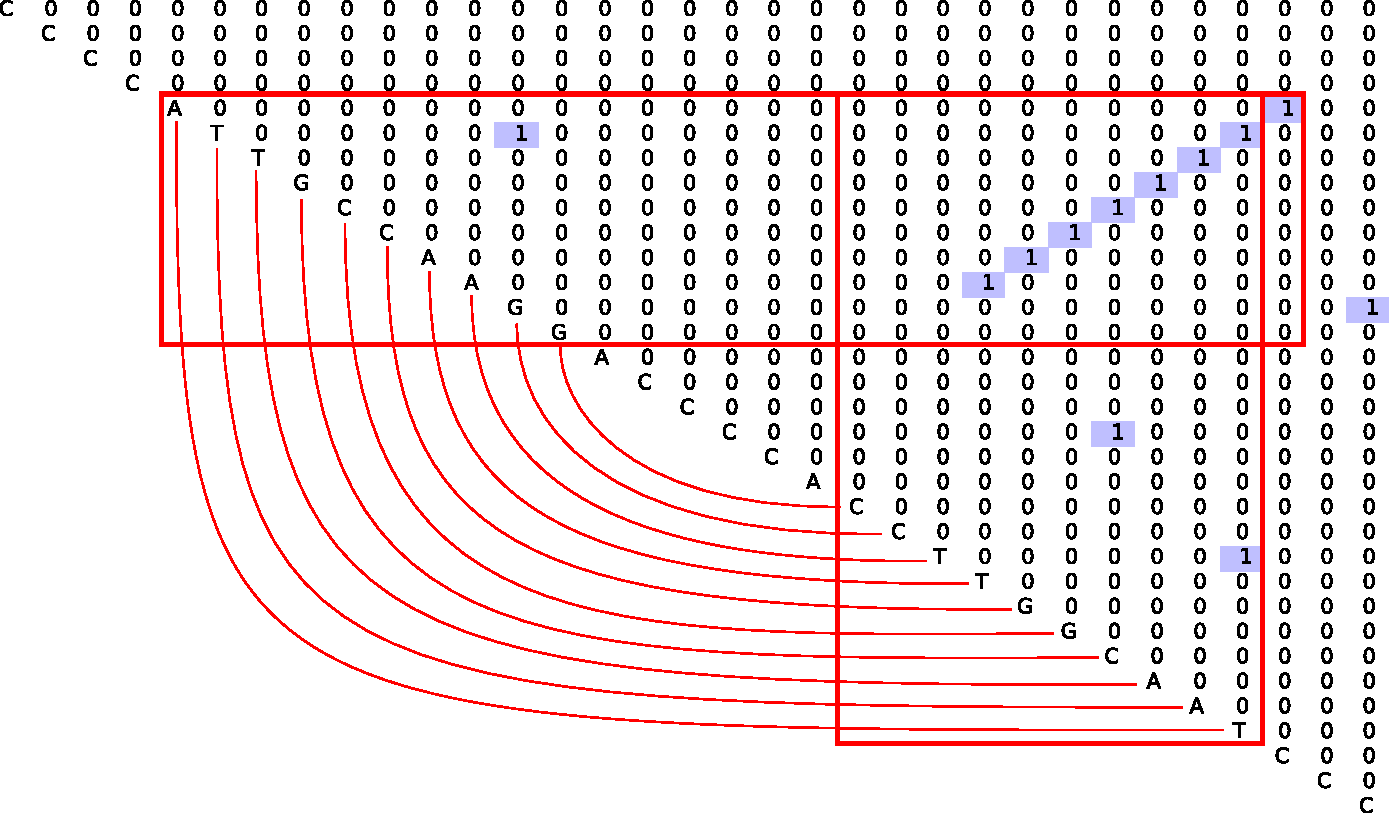
\includegraphics[width=0.8\textwidth]{figures/4.pdf}
\caption{Parsing result for sequence which should fold to
stem}
\label{fig:example}
\end{center}
\end{figure}

The parsing result in a form of a matrix can be linearized, compressed into a byte or int vector, and be further handled by a dense neural network, as described in~\cite{grigorevcomposition}.
Unfortunately, linearization breaks data locality: a diagonal chain of one-s, which signifies a high stem, is local in a matrix, but is broken apart during its linearization.
We see it to be an argument to investigate the applicability of convolutional networks for parsing result handling, as a boolean matrix can be converted to a black-white bitmap image.
In this paper, we provide an empirical comparison of networks which handle vectors and images.

Another problem is a bad performance of the earlier solution.
Since the trained network handles parsing result, each input sequence should first be parsed.
Parsing is a very time-consuming step: context-free parsing has cubic complexity in terms of the input length.
Even if we use matrix-based parsing algorithm~\cite{Azimov:2018:CPQ:3210259.3210264} which utilizes GPGPU, performance is insufficient.
We believe it would be better to avoid the parsing step at the final stage of the solution.
In this work, we propose a way to solve this problem by building a network which handles raw sequences, not parsing results.
